% Crucial Preamble
\documentclass[12pt,letterpaper]{article} \usepackage{amsmath} \usepackage{graphicx} \usepackage[margin=1in]{geometry} \usepackage{longtable}  \usepackage{amssymb}

% Extra Preamble
\usepackage{fancyhdr} \usepackage{enumitem} \usepackage{float} \usepackage{soul}
\usepackage{multicol} \usepackage[compact]{titlesec}
\usepackage[section]{placeins}
\usepackage{pdfpages}

% frames with display breaks
\usepackage{mdframed}
\allowdisplaybreaks

% change spacing
\usepackage{setspace}
\setlength{\parskip}{0.4\baselineskip}

% Remove paragraph indentation
\setlength{\parindent}{0pt}

% Reduce space before and after section headings
%\titlespacing*{\section}{0pt}{0.1\baselineskip}{0.2\baselineskip}

% changes font
%\renewcommand{\familydefault}{\sfdefault}

% adds header and footer
\pagestyle{fancy}
\fancyhead{} \fancyhead[C]{ELG 3125 Summary Sheet} \fancyhead[L]{ELG3125} \fancyhead[R]{Owen Daigle}
\fancyfoot{} \fancyfoot[C]{\thepage}


\begin{document}
	
	\begin{center}
		\Large\textbf{ELG 3125 Summary Sheet} \\
		\vspace{0.5em}
	\end{center}	

	\section{Basics of Signals and Systems}
	We can have a signal that is either continuous or discrete. These signals are represented as math functions.
	\begin{figure}[!h]
		\centering
		\includegraphics[width=0.8\linewidth]{"images/discrete vs cont"}
		\label{fig:discrete-vs-cont}
	\end{figure}
	Computers always will display and work with a discrete signal. However often it is to model a continuous signal. 
	
	We call a signal a power signal if its average power is finite. Similarly, we call a signal an energy signal if its total energy is finite. 
	
	\begin{mdframed}
		\textbf{Ex. } A 120VAC wall outlet is a power signal.
		
		This is because the average power is finite. If we have for example a 1500w heater connected, it will always draw 1500W. 
		
		However if we keep it running for a long time, it will use a very large amount of energy. So it is infinite energy.
	\end{mdframed} 
	
	\subsection{Transformations}
	There are many transformations.
	\begin{figure}
		\centering
		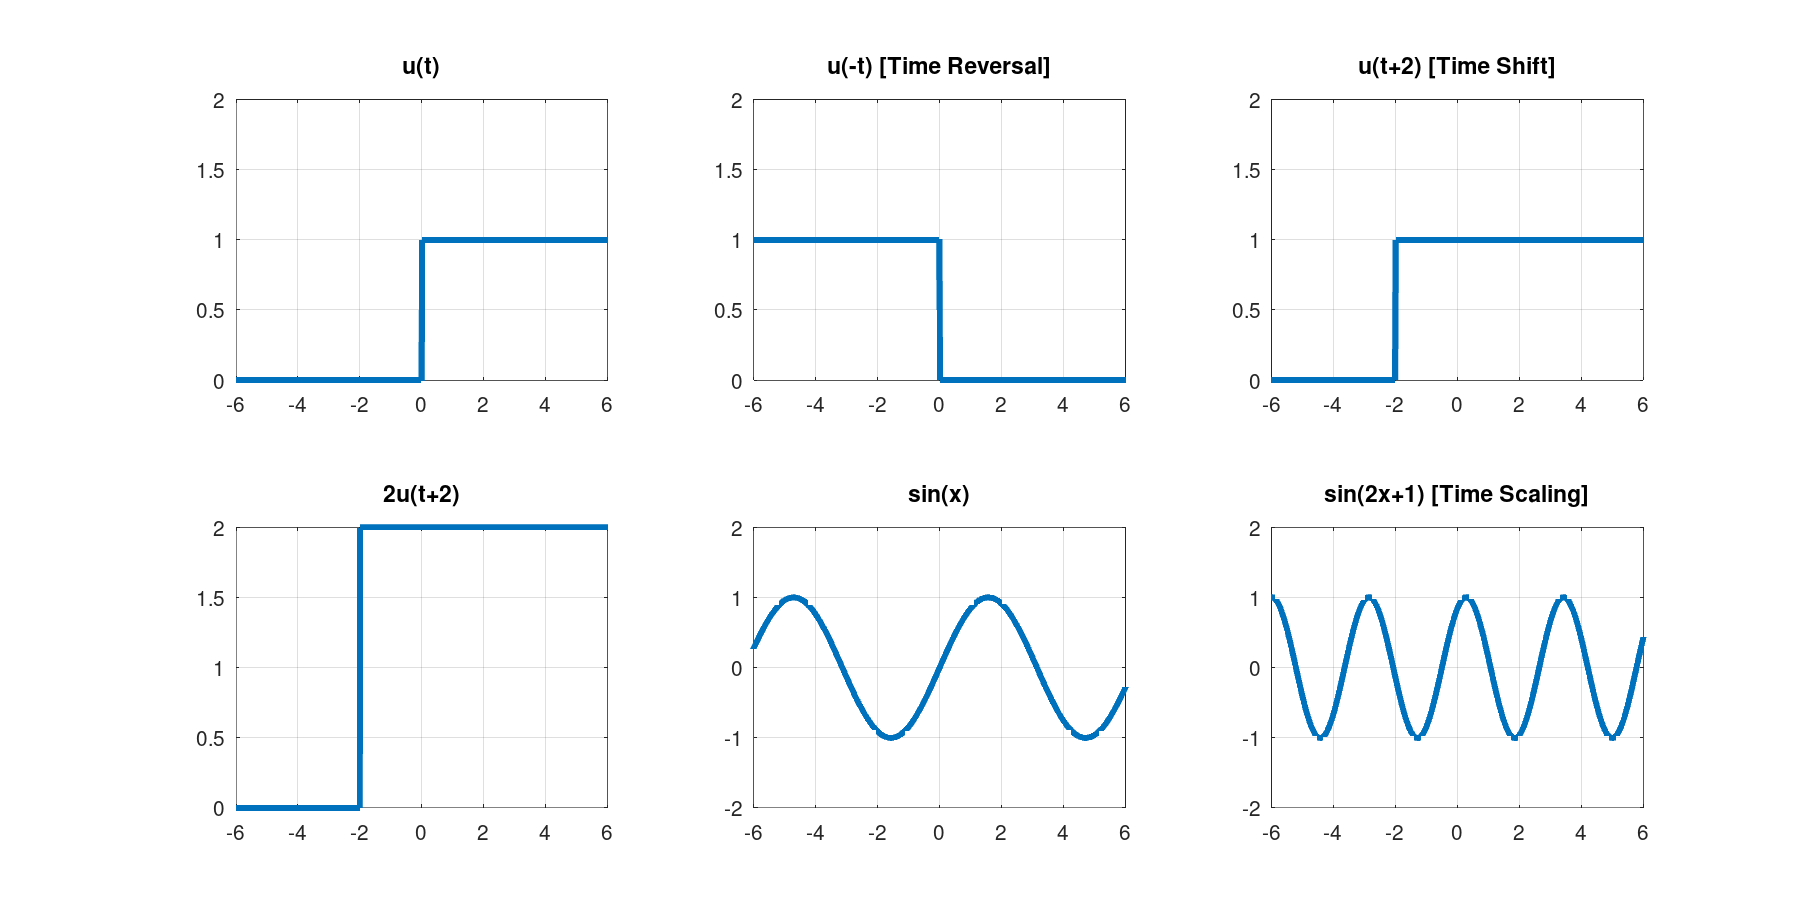
\includegraphics[width=0.8\linewidth]{images/transformations}

		\label{fig:transformations}
	\end{figure}
	
	When transforming a signal, we usually start with any time shifts. Then we apply other transformations such as a time reversal, or time scaling. 
	
	\begin{mdframed}
		\textbf{Ex. } Plot $\cos(-t/2 + 1)$
		
		We take it in 4 steps:
		
		\centering
		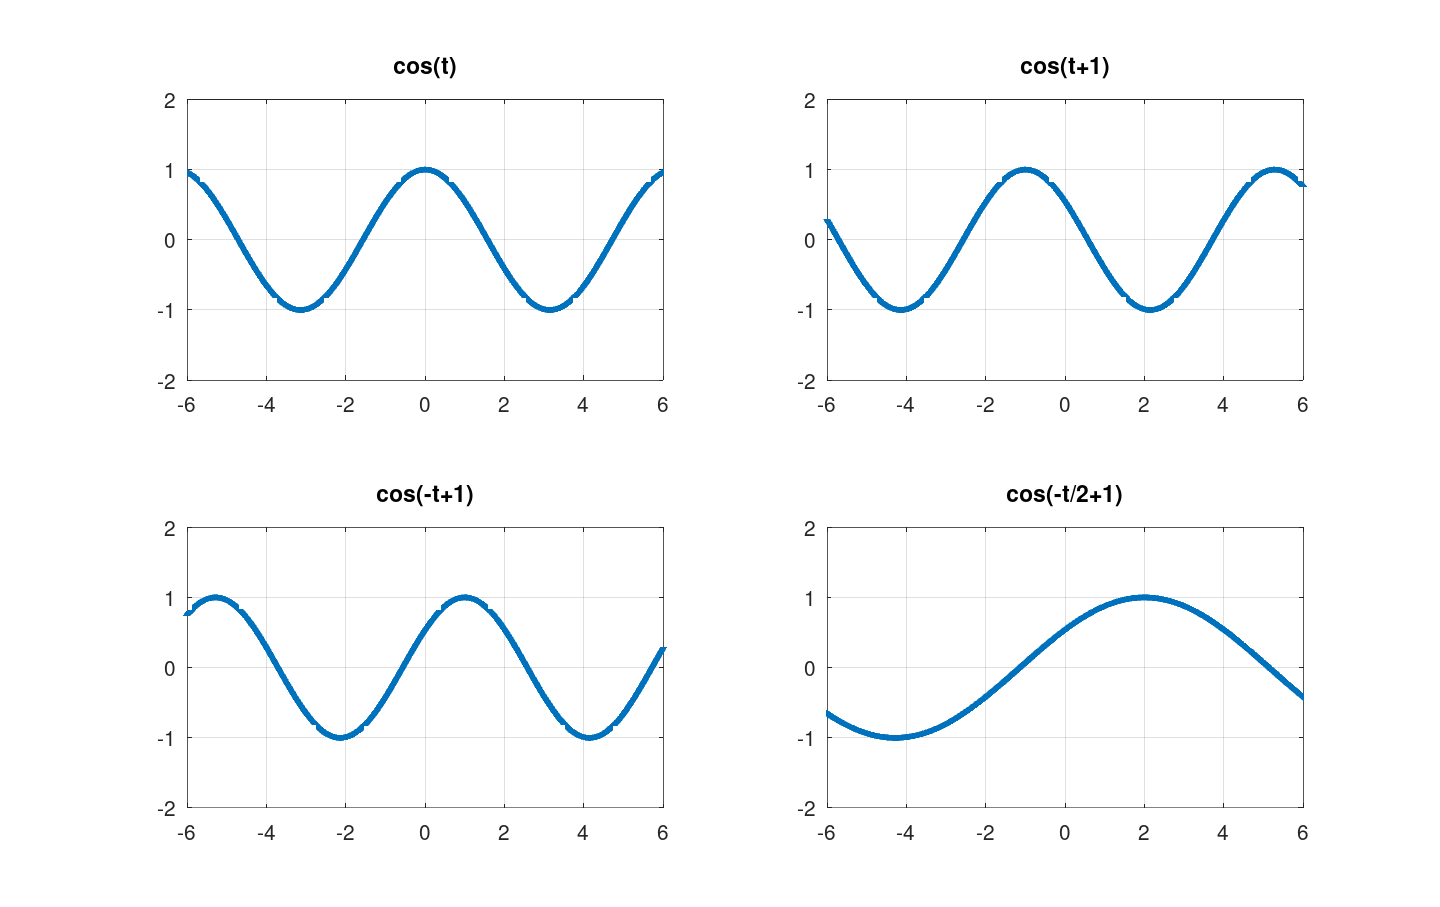
\includegraphics[width=0.8\linewidth]{images/ex1}
	\end{mdframed}
	
	\subsection{Periodicity}
	A signal is called periodic if:
	\begin{align}
		x(t) = x(t+T) \text{  } \forall \text{ }t\label{eq:1}
	\end{align}
	We call the fundamental period $T_0$ the smallest \textit{positive} value of $T$ for which Equation \ref{eq:1} holds.
	
	We have the same idea in discrete time except we change $t$ for $n$, and $T$ for $N$.
	\begin{align}
		x[n] = x[n+N] \text{  } \forall \text{ }n\label{eq:2}
	\end{align}
	
	Note that any complex exponential in the form of $e^{j\omega_0 t}$ is periodic with period $T = \frac{2\pi}{\omega_0}$.
	
	\begin{mdframed}
		\textbf{Ex.} Find the period of $x[n]$.
		\begin{align*}
			x[n] = e^{j(\frac{2\pi}{3})n} + e^{j(\frac{3\pi}{4})n}
		\end{align*}
		I need to find both periods, and find the greatest common multiple. 
		
		Note that since I am in discrete time, the period must be an integer. 
		\begin{align*}
			T_1 &= \frac{2\pi}{\frac{2\pi}{3}} = 3\\
			T_2 &= \frac{2\pi}{\frac{3\pi}{4}} = \frac{8}{3} = 8 \text{ since } \frac{8}{3} \notin \mathbb {Z}\\
			T &= LCM(3,8) = 24
		\end{align*}
	\end{mdframed}
	
	\subsection{Even and Odd Functions}
	We call a signal Even if it satisfies Equation \ref{eq:3} or Odd if it satisfies Equation \ref{eq:4}.
	\begin{align}
		x(t) = x(-t) \label{eq:3}\\
		x(t) = -x(-t) \label{eq:4}
	\end{align}
	We can construct any signal by using its even and odd portions. 
	\begin{align}
		x(t) = Ev\{x(t)\} + Od\{x(t)\} = \frac{1}{2}(x(t) + x(-t)) + \frac{1}{2} (x(t) - x(-t)) \label{eq:5}
	\end{align}
	
	\subsection{Unit Impulse and Unit Step}
	These are two very useful functions as defined below.
	\begin{figure}[!h]
		\centering
		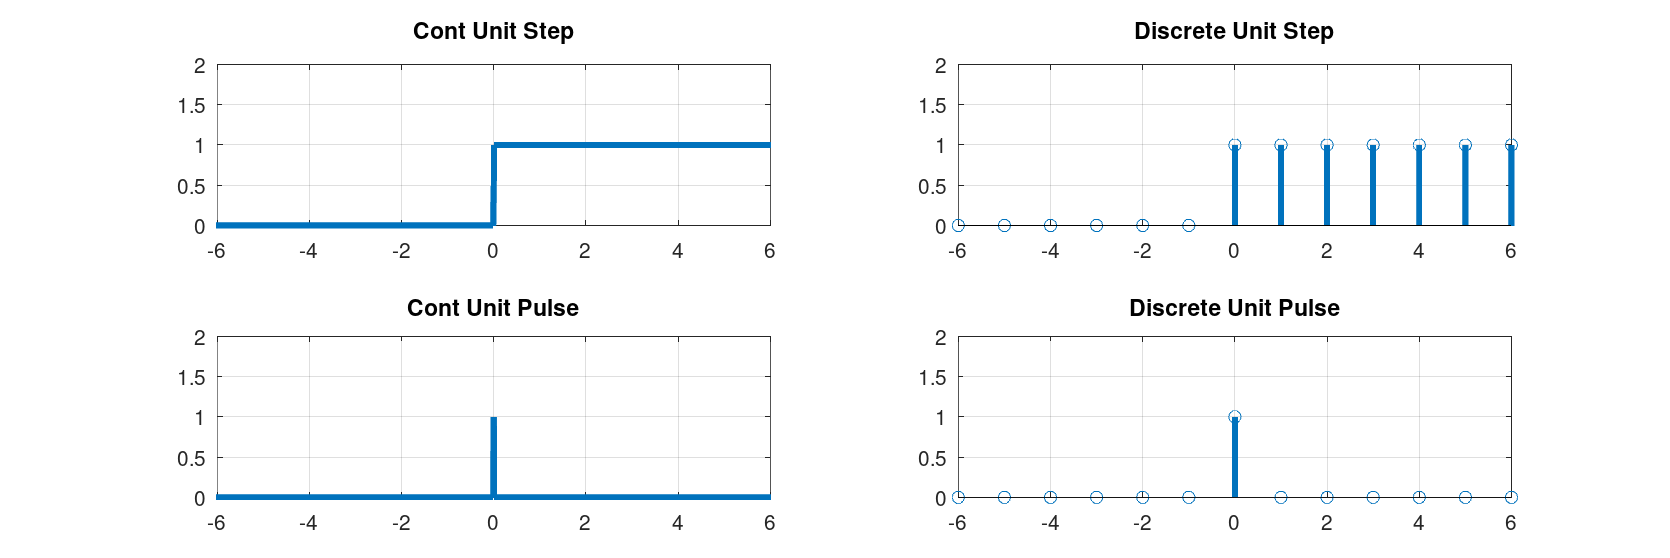
\includegraphics[width=0.9\linewidth]{images/unit step and impulse}
		
		\label{fig:unit}
	\end{figure}
	The unit step is 0 when x is negative, and 1 when positive or 0. The impulse is 1 only when x is 0.
	
	The unit step function is called $u(t)$ or $u[n]$. The unit pulse is called $\delta(t)$ or $\delta[n]$.
	
	\subsection{System Properties}
	
	\subsubsection{Memory}
	A system is memoryless if the output is only dependant on the input at the same time. 
	
	So basically we do not see any time shifts such as $t-1$ or $t+1$.
	
	\subsubsection{Invertibility}
	A system is invertible if distinct inputs lead to distinct outputs. 
	
	\begin{mdframed}
		\textbf{Ex.} Example found in 
	\end{mdframed}
	
	\subsubsection{Causality}
	A system is causal if the output at any time depends only on input values of present and in the past. It does not depend on any future values. 
	
	This is also referred to as being nonanticipative.
	
	Note that all memoryless systems are causal.
	
	Basically if we see something like $x(t+1)$, it is non causal. If we see something like $(t+1) x(t)$, it is likely causal. 
	
	\subsubsection{Stability}
	A system is stable if when inputs are bounded, the outputs are always bounded. So:
	\begin{align}
		|x(t)| < \infty \implies |y(t)| < \infty 
	\end{align}
	Assuming $x(t)$ is input, and $y(t)$ is output.
	
	\subsubsection{Time Invariance}
	A system is time invariant if a time shift in the input results in an identical time shift in the output. 
	
	\begin{mdframed}
		\textbf{Ex.} Is y(t) = x(6t) time invariant?
		
		We can do:
		\begin{align*}
			y(t-t_0) &= x(6t-6t_0) \qquad \text{Now we delay by $-t_0$}\\
			y(t) &= x(6t-5t_0)  \qquad \text{Now we delay by $+t_0$}\\
			&\ne x(6t) \qquad \text{So it is NOT time invariant.}
		\end{align*}
	\end{mdframed}

	
	\subsubsection{Linearity}
	A system is linear if Equation \ref{eq:6} is satisfied.
	\begin{align}
		ax_1 (t) + bx_2 (t) \to ay_1 (t) + by_2(t)\label{eq:6}
	\end{align}
	
	\begin{mdframed}
		\textbf{Ex. } Is $y(t) = x(t)^2$ linear?
		
		We know intuitively that the answer is no here. But we can prove this using the relation:
		\begin{align*}
			y_1(t) &= x_1(t)^2\\
			y_2(t) &= x_2(t)^2\\
			x_3(t) &= ax_1(t) + bx_2(t)\\
			y_3(t) &= ay_1(t) + by_2(t)\\
			y_3(t) = ax_1(t)^2 + bx_2(t)^2 &\ne \left[ax_1(t) + bx_2(t)\right]^2 = x_3(t)^2
		\end{align*}
		Basically what we did here is find the left side of the equation by finding the output twice, vs finding the left side by doing the input twice. 
	\end{mdframed}
	
	\begin{mdframed}
		\textbf{Ex. } Find all the properties of $y(t) = \cos(t)x(t+1)$.
		
		We see that it is with memory since it relies on $t+1$.
		
		It is not causal since it depends on a future value $t+1$.
		
		If we have an input that is finite, so $x(t) < \infty$, then we also have $\cos(t) < \infty$ since $-1 \ge \cos(x)\ge 1$.
		
		To determine if it is time variant, we need to do $t = t-t_0$ and then remove the $t_0$ from each side. We see if we are still the same.
		\begin{align*}
			y(t-t_0) &= \cos(t-t_0)x(t+1-t_0)\\
			\implies \qquad  y(t) &= \cos(t-t_0) x(t+1) \qquad\qquad  X
		\end{align*}
		So it is not time invariant. 
		To see if it is linear we check the equation. 
		\begin{align*}
			y_1(t) &= \cos(t)x_1(t+1)\\
			y_2(t) &= \cos(t) x_2(t+1)\\
			y_3(t) &= y_1(t) + y_2(t) =  \cos(t)x_1(t+1) +  \cos(t)x_2(t+1) \\&= \cos(t) \left[x_1(t+1) + x_2(t+1)\right] = ay_1(t) + by_2(t)
		\end{align*}
	\end{mdframed}
	
	
	
	\section{LTI Systems}
	Many systems in the real world are linear and time invariant. An example is a signal amplifier. 
	
	\subsection{Convolution in Discrete Time}
	The convolution sum contains 3 parts. 
	\begin{itemize}
		\item $h[n]$ is the response of the LTI system
		\item $x[n]$ is the input to the LTI system
		\item $y[n]$ is the output of the LTI system
	\end{itemize}
	
	\begin{mdframed}
		\textbf{Ex.} Consider a signal amplifier such as a microphone amplifier, or a speaker amplifier. 
		
		If we have a microphone or speaker, the input $y[n]$ is the input such as the voice or the demodulated radio signal. 
		
		The response $h[n]$ is the algorithms that do all the amplification, and maybe some noise reduction. 
		
		The output $y[n]$ is the final audio signal such as what we hear from a speaker. 
	\end{mdframed}
	
	The convolution sum is how we calculate the output given an input and response. We can think of this as we have the response $h[n]$, and then we send through the input $x[n]$ throughout the entire response. 
	\begin{figure}
		\centering
		\includegraphics[width=0.7\linewidth]{"images/convolution idea"}
		\label{fig:convolution-idea}
	\end{figure}
	
	The convolution is represented in Equation \ref{eq:7}.
	\begin{align}
		y[n] = \sum^{\infty}_{k=-\infty} x[k]h[n-k] = x[n]*h[n] \label{eq:7}
	\end{align}
	Note that when finding the convolution, we now consider $k$ as the x axis variable, and $n$ as a constant. 
	
	To calculate the convolution sum, we draw $h[n-k]$ and $x[k]$. Then we analyze all overlap regions and find $x[k]\cdot h[n-k]$ for that region. 
	
	\subsection{Convolution in Continuous Time}
	This is very similar to the convolution in discrete time except now we have $h(t), y(t), x(t)$. We also use an integral to calculate the convolution instead of a sum as shown in Equation \ref{eq:8}.
	\begin{align}
		y(t)=\int^{\infty}_{-\infty} x(\tau)h(t-\tau)\mathrm d\tau = x(t)*h(t)\label{eq:8}
	\end{align}
	
	Again to solve, we break it up into all the overlap regions and find the product ($x(t)\cdot h(t)$) for each region.
	
	\begin{mdframed}
		\textbf{Ex.} We have a system response $h(t)$. The input $x(t) = \delta(t)$. What is the output $y(t)$?
		
		This is very simple. We could go about calculating the convolution sum using equation \ref{eq:8}, but we can also think this through logically. 
		
		Recall that the response $h(t)$ is just the stuff that is applied to the input signal $x(t)$. Since the input signal is just a single pulse, it will travel through the system visiting each point only \textbf{once}. 
		
		This means that the output will just be the response. 
		\begin{align*}
			y(t) = x(t) * h(t) = \delta(t) * h(t) = h(t)
		\end{align*}
		This is actually a general equation where:
		\begin{align}
			x(t)*\delta(t-t_0) = x(t-t_0)
		\end{align}
	\end{mdframed}
	
	\begin{mdframed}
		\textbf{Ex. } We have an input signal and a convolution. Find the output.
		\begin{align*}
			x(t) = \delta (t-1) + e^{-3t} u(t) \qquad h(t) = u(t-1) - u(t-5)
		\end{align*}
		To find the output, I need to take the convolution of these two signals. I will need to plot $h(-k+n)$, and it will be helpful to have a plot of the input as well.
		
		I see that $x(t)$ looks complicated to plot. So I will do it in two plots. 
		
		\centering
		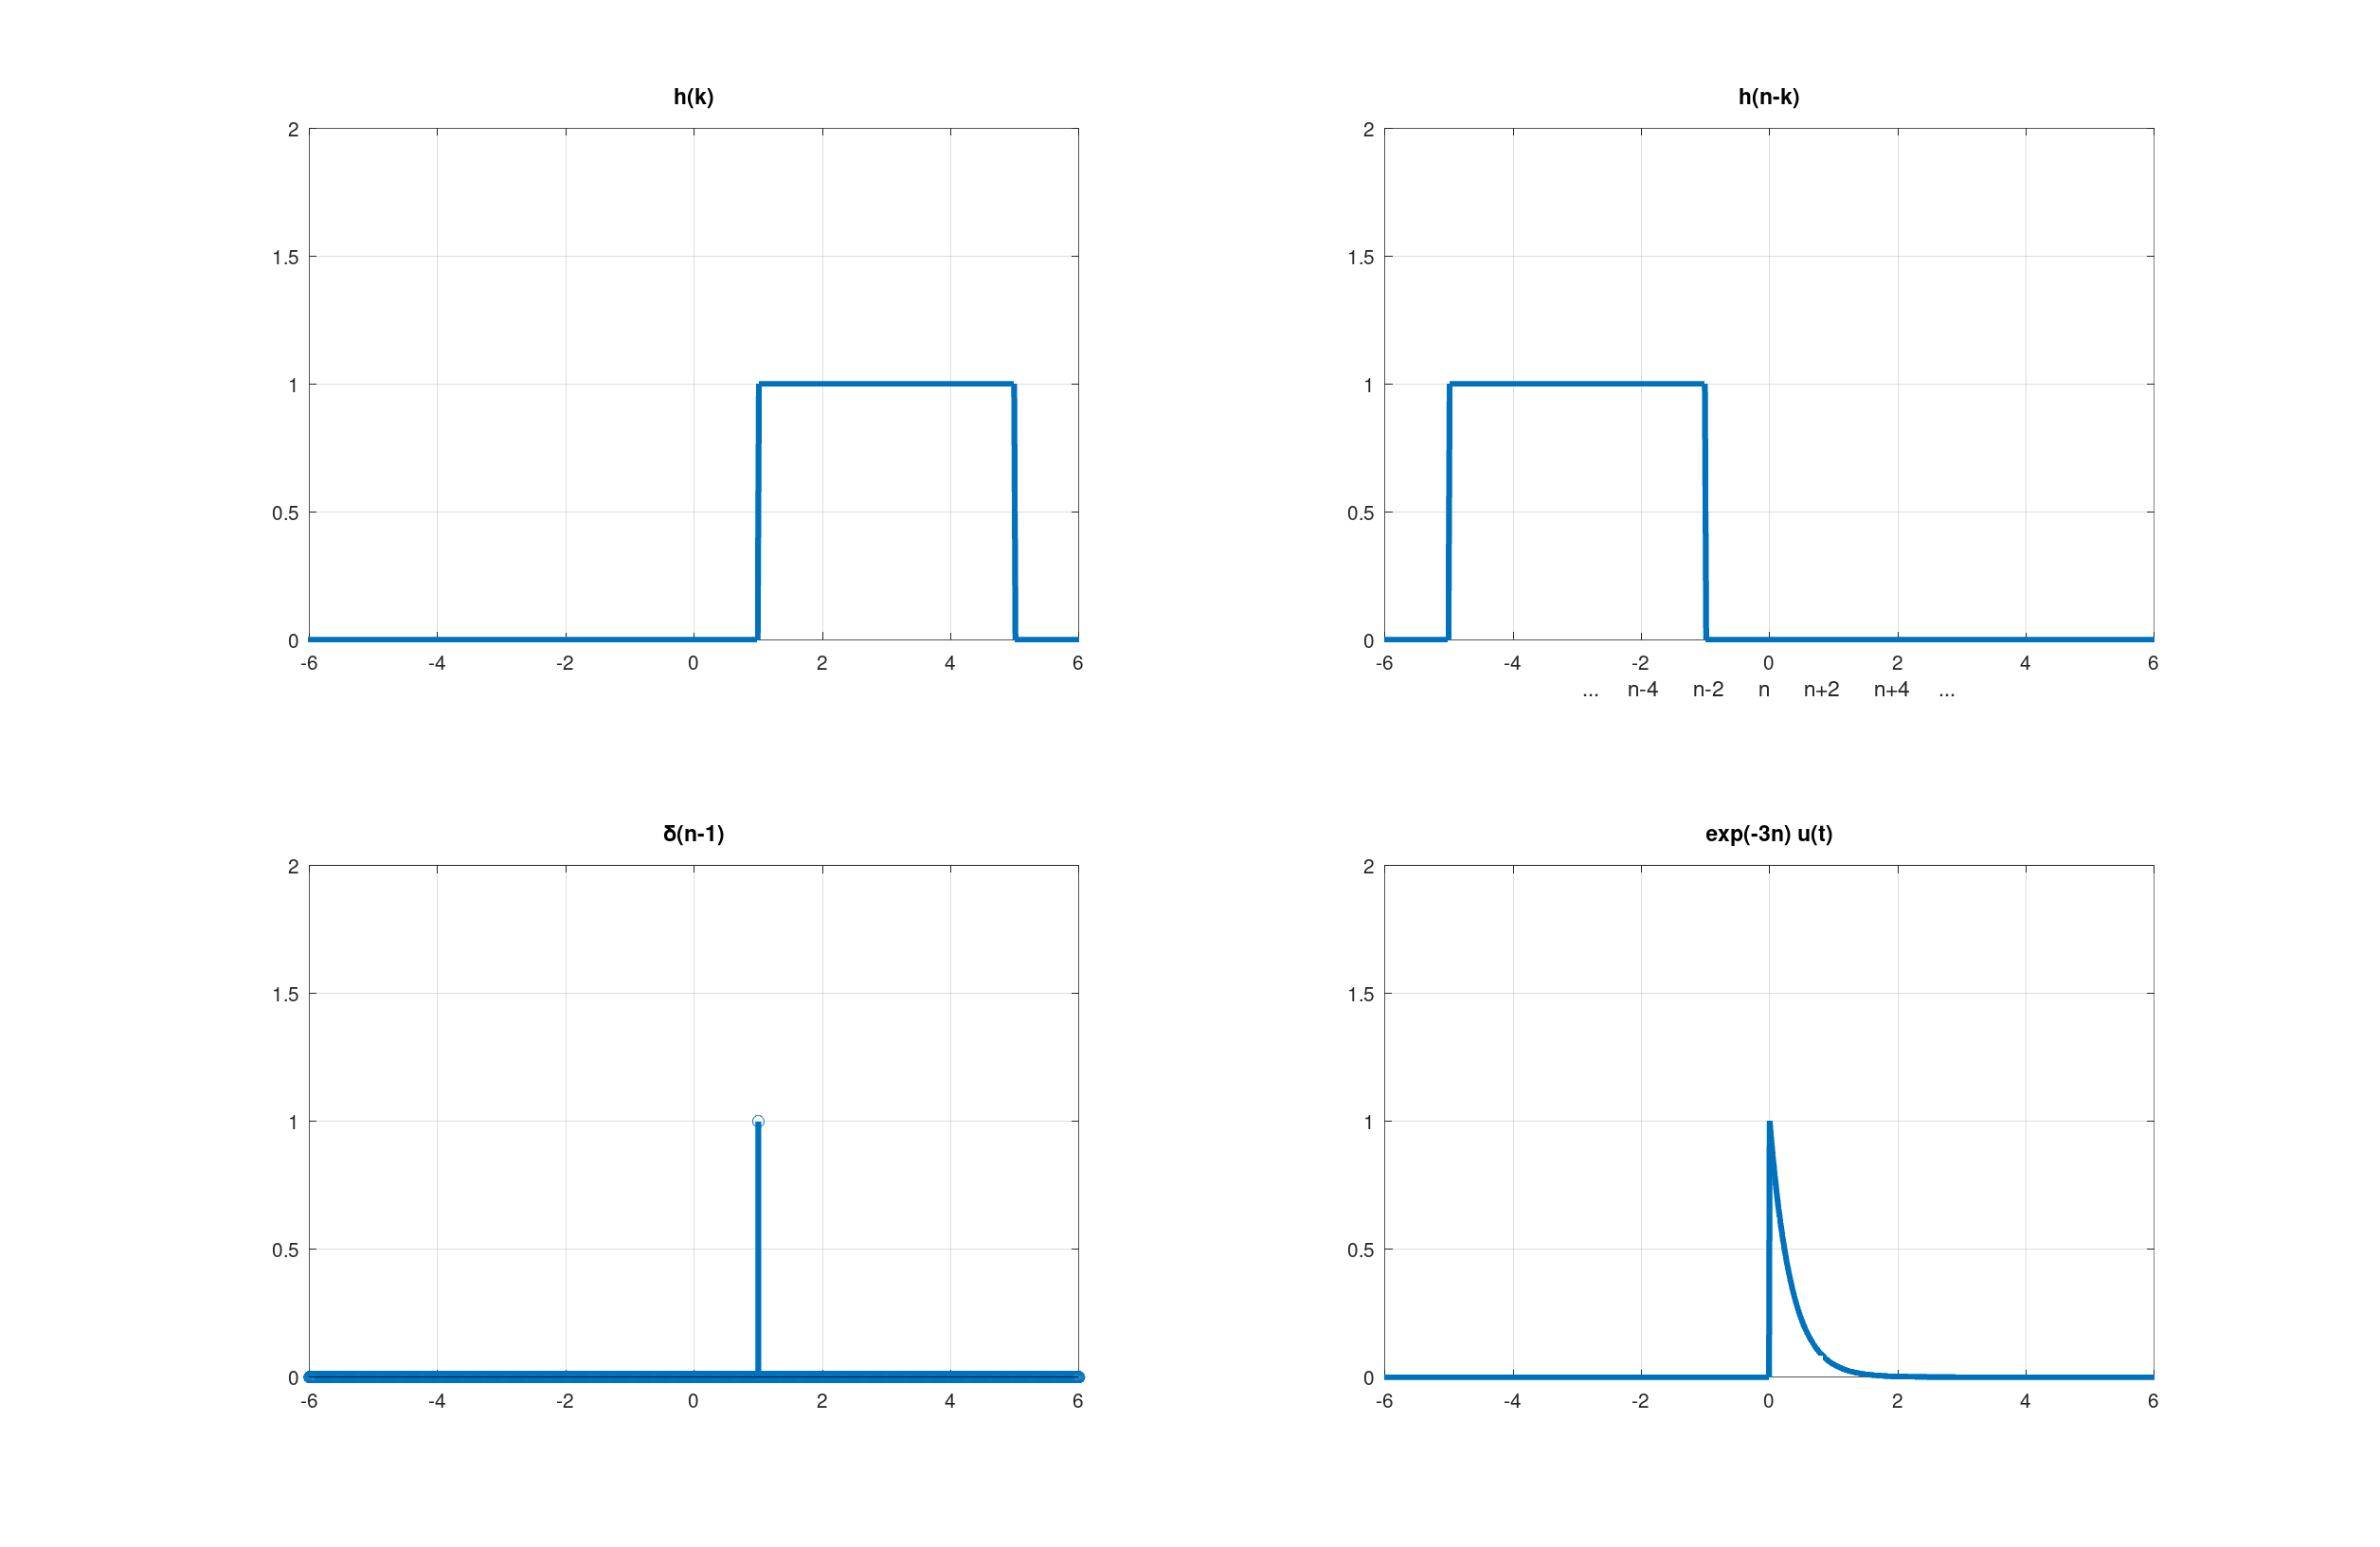
\includegraphics[width=0.99\linewidth]{images/ex3}

		\raggedright
			
		Now we need to run the response $h(n-k)$ through both other functions.
		
		Note that k is the variable that we change. So we change 
		
		Using the first delta function, I have 3 areas:
		\begin{align*}
			&n-1<1 \implies n<2 & =0\\
			&1 < n-1 < 5 \implies 2 < n < 6 & =1\\
			&n-1 > 5 \implies n > 6 & =0
		\end{align*}
		Then for the second function, I also have 3 regions. 
		\begin{align*}
			& k -1 < 0 \implies k<1 & = 0\\
			&0 < k-1 < 4 \implies 1 < k < n & \int_1^{n} e^{-3(t-k)}\mathrm d k = e^{-3t} \int_1^n e^{3k} \mathrm d k\\
			&k-1 > 4 \implies k > 5 & =0
		\end{align*}
		Now we can add up the 2 functions to get 5 regions. 
	\end{mdframed}
	
	\subsection{Properties}
	An LTI system is memoryless if $h[n] = K\delta[n]$ where $k \in \mathbb R$. This means $y[n] = Kx[n]$.
	
	An LTI system is invertable if we can get back the input after applying a convolution to the output. 
	\begin{figure}[H]
		\centering
		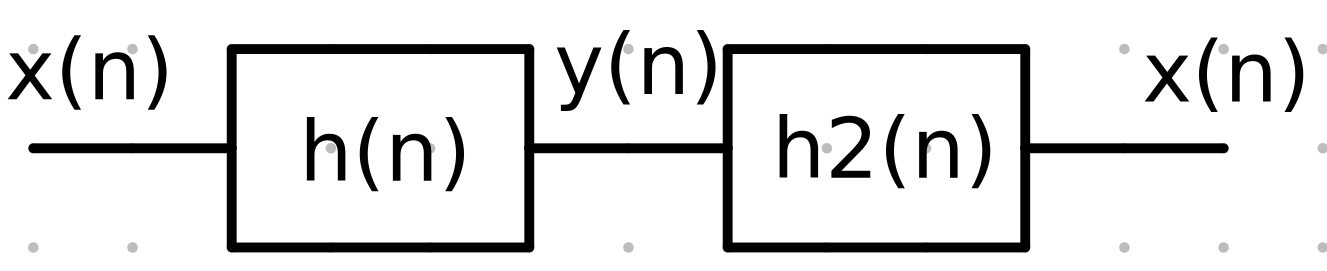
\includegraphics[width=0.4\linewidth]{images/invertability}
		\label{fig:invertability}
	\end{figure}
	
	An LTI system is causal if $h[n] = 0$ for $n < 0$.
	
	An LTI system is stable if for all finite inputs to the response, the output os finite: $\int^{\infty}_{-\infty} |h(t)|\mathrm d \tau < \infty$.
	\subsection{Differential and Difference Equations}
	These are equations in the form of:
	\begin{align*}
		y[n] = y[n-1] + x[n] \qquad \text{Difference Equation}\\
		\frac{dy(t)}{dt} + y(t) = x(t) \qquad \text{Differential Equation}
	\end{align*}
	We can solve difference equations by using the initial rest condition which is a time when the output is 0. Then we can solve for consecutive values of $n$ starting at initial rest. 
	
	For differential equations we need to find the homogeneous solution (input is 0) and the particular solution. Then we sum them together. 
	
	\begin{mdframed}
		\textbf{Ex. } We have a causal LTI system described by $y[n] - \frac{1}{3} y[n-1] = x[n]$
		
		The impulse response $h[n]$ can be found by remembering that if we let $x[n] = \delta[n]$ then $y[n]=h[n]$.
		\begin{align*}
			h[n] = \delta[n] + \frac{1}{3} h[n-1]
		\end{align*}
		Then since it is causal, we know that when $n<0$, $h[n]=0$. So I can try a few values to get a pattern.
		\begin{align*}
			h[0] &= \delta[0] + \frac{1}{3}h[-1] = 1 + \frac{1}{3} (0) = 1\\
			h[1] &= \delta[1] + \frac{1}{3}h[0] = \frac{1}{3} (1) = \frac{1}{3}\\
			h[2] &= 0 + \frac{1}{3} \frac{1}{3} = \left[\frac{1}{3}\right]^2\\
			h[3] &= \left[\frac{1}{3}\right]^3\\
			h[n] &= \left[\frac{1}{3}\right]^n
		\end{align*}
		Now we know $h[n]$. We can do many things. 
		
		We know the system is stable since if we increase $n \to \infty$ then $h[n]$ is finite. 
		
		We also can find the inverse impulse response $h'[n]$ by just swapping $x$ for $y$ in the original equation and then solving using the same method. 
		
		If we want to find the output given a certain input we can. We just use the convolution sum to do so. We would end up with three regions, the first of which $y[n]=0$.
	\end{mdframed}
	
	\begin{mdframed}
		\textbf{Ex. } % put differential equation example here
	\end{mdframed}
	\section{Fourier Series}
	Any periodic signal can be represented by sinusoids (or complex exponentials).
	
	We have the signal of $e^{j\omega_0t}$ which is periodic. It contains both sin and cos components. 
	
	If we change it to $e^{jk\omega_0 t}$, for $k=0, \pm1, \pm2, ...$ then we say that these are harmonically related. The first harmonic has $k=\pm1$, the second $k=\pm2$, and so on. We have:
	\begin{align}
		x(t) = a_0 + \sum^{\infty}_{k=1} \left[a_k e^{jk\omega_0t} + a_{-k}e^{-jk\omega_0t}\right]
	\end{align}
	
	We see that the $e$ terms are constant, only the coefficients change a meaningful amount. We can calculate the coefficients using Equation \ref{eq:9}.
	\begin{align}
		a_k &= \frac{1}{T}\int^T_0 x(t)e^{-jk\omega_0 t}\mathrm d t\label{eq:9}\\
		a_0 &= \frac{\text{AREA}}{T} \qquad \text{Specific Case for DC offset ($a_0$)}
	\end{align}
	
	\begin{mdframed}
		\textbf{Ex.} Find $a_k$ and $a_0$
		
		\centering
		
		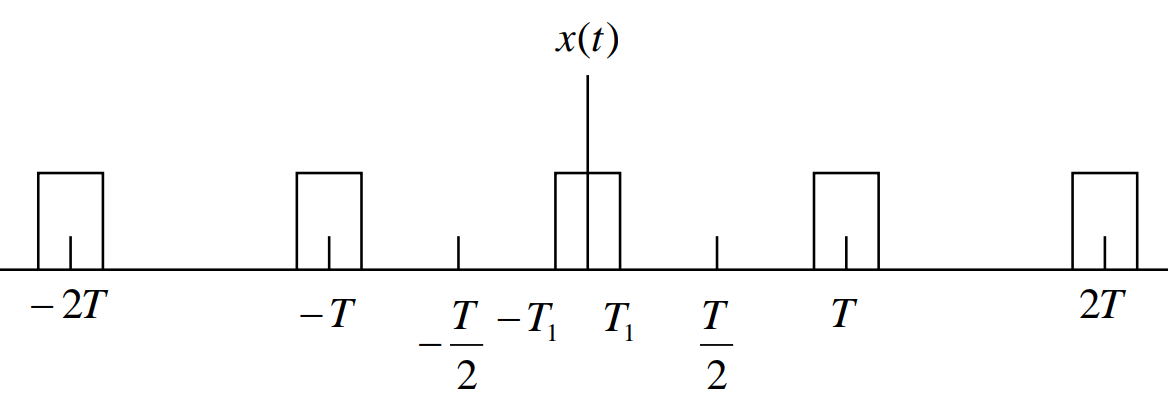
\includegraphics[width=0.7\linewidth]{images/ex2}
		
		\raggedright
		We need to use Equation \ref{eq:9}.
		\begin{align*}
			a_k &= \frac{1}{T}\int^T_0 x(t)e^{-jk\omega_0 t}\mathrm d t = \frac{1}{T}\int^{-T_1}_{T_1} 1\cdot e^{-jk\omega_0 t}\mathrm d t = \frac{1}{Tjk\omega_0}e^{-jk\omega_0 t}|^{T_1}_{-T_1} = \frac{2}{k\omega_0 T}\left[\frac{e^{jk\omega_0 T_1 - e^{-jk\omega_0 T_1}}}{2j}\right]\\
			&= \frac{2}{k\omega_0T}\cdot \sin(k\omega_0T_1) \qquad \text{Using an identity} \\
			a_k&= \frac{\sin(k\omega_0 T_1)}{k\pi} \qquad \text{Using $T = \frac{2\pi}{\omega_0}$}\\
			\\
			a_0 &= \frac{\text{AREA}}{T} = \frac{2T_1}{T} \qquad \text{We could also use $a_k$ to get 0/0, and use l'Hopital}
		\end{align*}
		
	\end{mdframed}
	
	\subsection{Properties of Continuous Fourier Series}
	If we have coefficients $a_k$ already for a signal $x(t)$, or maybe more than one signal $x(t)$ and $y(t)$, then after applying some changes to the signals we come up with new coefficients by these properties.
	\begin{center}
		\begin{tabular}{|c||c|c|}
			\hline
			Property & Periodic Signal & Coefficients \\
			\hline\hline
			Linearity & $A x(t) + B y(t)$ & $A a_k + B b_k$ \\
			\hline
			Time Shifting & $x(t-t_0)$ & $e^{-jk\omega_0 t_0} a_k$ \\
			\hline
			Frequency Shifting & $e^{jM\omega_0 t} x(t)$ & $a_{k-M}$ \\
			\hline
			Conjugation & $x^*(t)$ & $a^*_{-k}$ \\
			\hline
			Time Reversal & $x(-t)$ & $a_{-k}$ \\
			\hline
			Time Scaling & $x(\alpha t), \ \alpha > 0$ & $a_k$ \\
			\hline
			Periodic Convolution & $\int_T x(\tau) y(t-\tau) \mathrm{d}\tau$ & $T a_k b_k$ \\
			\hline
			Multiplication & $x(t) y(t)$ & $\sum^{\infty}_{l=-\infty} a_l b_{k-l}$ \\
			\hline
			Differentiation & $\frac{\mathrm{d} x(t)}{\mathrm{d} t}$ & $j k \omega_0 a_k = j k \frac{w \pi}{T} a_k$ \\
			\hline
			Parseval's Relation & $\frac{1}{T} \int_T |x(t)|^2 \mathrm{d} t = \sum^{\infty}_{k=-\infty} |a_k|^2$ &  \\
			\hline
		\end{tabular}
	\end{center}
	
	
	\subsection{Properties of Discrete Fourier Series}
	It is the same idea with discrete signals. We have the equations for the coefficients, and the properties. 
	
	\begin{align}
		x[n] = \sum_{k=N} a_k e^{jk\omega_0 n}\\
		a_k = \frac{1}{N} \sum _{n=N} x[n]e^{-jk\omega _0}n
	\end{align}
	
	\begin{center}
		\begin{tabular}{|c||c|c|}
			\hline
			Property & Periodic Signal & Coefficients \\
			\hline\hline
			Linearity & $A x[n] + B y[n]$ & $A a_k + B b_k$ \\
			\hline
			Time Shifting & $x[n-n_0]$ & $e^{-jk\omega_0 n_0} a_k$ \\
			\hline
			Frequency Shifting & $e^{jM\omega_0 n} x[n]$ & $a_{k-M}$ \\
			\hline
			Conjugation & $x^*[n]$ & $a^*_{-k}$ \\
			\hline
			Time Reversal & $x[-n]$ & $a_{-k}$ \\
			\hline
			Time Scaling & $x_m[n]$ & $a_k$ \\
			\hline
			Periodic Convolution & $\sum_{r=N} x[r] y[n-r]$ & $N a_k b_k$ \\
			\hline
			Multiplication & $x[n] y[n]$ & $\sum_{l=N} a_l b_{k-l}$ \\
			\hline
			Differentiation & $x[n] - x[n-1]$ & $(1-e^{-jk\omega_0})a_k$ \\
			\hline
			Parseval's Relation & $\frac{1}{T} \sum_{n=N} |x[n]|^2 = \sum_{n=N} |a_k|^2$ &  \\
			\hline
		\end{tabular}
	\end{center}
	
	% MIDTERM MATERIAL ENDS HERE
	\section{Fourier Transformations}
	We can also represent non periodic (aperiodic) signals by sinusoids using Fourier Transformations.
	
	We do this by taking a periodic signal, and increasing the period to be very large. This makes it so each pulse of the periodic signal is infinitesimally far apart, which means it is basically a non periodic signal.
	
	We can represent a signal in either the time domain (what we usually do) or the frequency domain. The frequency domain is similar to the fourier series representation of a periodic function. 
	\begin{align}
		x(t) &= \frac{1}{2\pi} \int_{-\infty}^\infty X(\jmath \omega) e^{\jmath\omega t}\mathrm d \omega \qquad \text{Time Domain (Inverse Fourier Transform)} \\
		x(\jmath \omega) &= \int^\infty_{-\infty} x(t) e^{-\jmath \omega t}\mathrm d t \qquad \text{Frequency Domain (Fourier Transform)}
	\end{align} 
	
	We can also fourier transform periodic signals into the frequency domain using:
	\begin{align}
		X(\jmath \omega) = \sum^\infty_{-\infty}2\pi a_k \delta(\omega - k\omega_0)
	\end{align}
	
	These are some common fourier transform pairs:
	\[
	\begin{array}{|c|c|}
		\hline
		e^{-a t} u(t) \quad \Longleftrightarrow \quad \frac{1}{a + j\omega},\quad a>0 &
		e^{-a|t|} \quad \Longleftrightarrow \quad \frac{2a}{a^2 + \omega^2},\quad a>0 \\
		
		\hline
		x(t) = \left\{
		\begin{array}{ll}
			1, & |t| < T_1 \Longleftrightarrow \frac{2\sin\omega T_1}{\omega} \\
			0, & |t| > T_1 \Longleftrightarrow \frac{2\sin\omega T_1}{\omega}
		\end{array}
		\right. &
		\frac{\sin Wt}{\pi t} \Longleftrightarrow X(j\omega) = 
		\left\{
		\begin{array}{ll}
			1, & |\omega| < W \\
			0, & |\omega| > W 
		\end{array}
		\right. \\
		
		\hline
		\delta(t) \Longleftrightarrow 1 & \delta(t-t_0) \Longleftrightarrow e^{-j\omega t_0} \\
		
		\hline
		1 \Longleftrightarrow 2\pi \delta(\omega) & e^{j\omega_0 t} \Longleftrightarrow 2\pi\delta(\omega-\omega_0) \\
		
		\hline
		\sin\omega_0 t \Longleftrightarrow \frac{\pi}{j}\delta(\omega-\omega_0) - \frac{\pi}{j}\delta(\omega+\omega_0) &
		\cos\omega_0 t \Longleftrightarrow \pi\delta(\omega-\omega_0) + \pi\delta(\omega+\omega_0) \\
		
		\hline
		\sum_{k=-\infty}^{\infty} a_k e^{j k \omega_0 t} \Longleftrightarrow \sum_{k=-\infty}^{\infty} 2\pi a_k \delta(\omega - k \omega_0) &
		\sum_{k=-\infty}^{\infty}\delta(t - kT) \Longleftrightarrow \frac{2\pi}{T} \sum_{k=-\infty}^{\infty} \delta\left(\omega - \frac{2\pi k}{T_0}\right) \\
		
		\hline
	\end{array}
	\]
	
	\subsection{Properties}
	We also have a lot of properties of these transforms such as the derivative which is very useful.
	
	Below is a table with some of the ones:
	\begin{center}
		\begin{tabular}{|c|c|}
			\hline
			Time Shifting & $x(t-t_0) \Longleftrightarrow e^{-j\omega t_0} X(j\omega)$ \\
			\hline
			Time Reversal & $x(-t) \Longleftrightarrow X(-\jmath\omega)$\\
			\hline
			Time and Frequency Scaling & $x(\alpha t) \Longleftrightarrow \frac{1}{|\alpha|} X\left(\frac{\jmath \omega}{\alpha}\right)$\\
			\hline
			Conjugate & $x^*(t) \Longleftrightarrow X^*(-j\omega)$ \\
			\hline
			Differentiation & $\frac{\mathrm{d}x(t)}{\mathrm{d}t} \Longleftrightarrow j\omega X(j\omega)$ \\
			\hline
			Parseval's Relation & $\int_{-\infty}^{\infty} |x(t)|^2 \mathrm{d}t \Longleftrightarrow \frac{1}{2\pi} \int_{-\infty}^{\infty} |X(j\omega)|^2 \mathrm{d}\omega$ \\
			\hline
			Convolution & $y(t) = h(t) * x(t) \Longleftrightarrow Y(j\omega) = H(j\omega) X(j\omega)$ \\
			\hline
			Multiplication & $r(t) = s(t)p(t) \Longleftrightarrow R(j\omega) = \frac{1}{2\pi} \int_{-\infty}^{\infty} S(j\theta) P(j(\omega-\theta)) \mathrm{d}\theta$ \\
			\hline
		\end{tabular}
	\end{center}
	
	
	\section{Discrete Time Fourier Transformation}
	This is very similar to the fourier transforms in continuous time, but there are slight differences. 
	
	The idea is exactly the same, it is just a few equations that we use are a bit different.
	
	We get the two equations of:
	\begin{align}
		x[n] &= \frac{1}{2\pi} \int_{2\pi} X(e^{j\omega}) e^{\jmath \omega n} \mathrm d \omega \qquad \text{Time Domain (Inverse Fourier Transform)} \\
		x[e^{\jmath \omega}] &= \sum^\infty_{n=-\infty} x[n]e^{-j\omega n} \qquad \text{Frequency Domain (Fourier Transform)}
	\end{align} 
	
	\begin{tabular}{|c|c|}
		\hline
		
		$\delta[n] \Longleftrightarrow 1$ & $a^n u[n], |a| < 1 \Longleftrightarrow \frac{1}{1 - a e^{-j\omega}}$ \\
		
		\hline
		
		$a^{|n|}, |a| < 1 \Longleftrightarrow \frac{1-a^2}{1-2a\cos\omega + a^2}$ & $x[n] = \begin{cases} 1, & |n| \leq N_1 \\ 0, & |n| > N_1 \end{cases} \Longleftrightarrow \frac{\sin \omega (N_1 + 1/2)}{\sin(\omega / 2)}$ \\
		
		\hline
		
		$e^{j\omega_0 n} \Longleftrightarrow 2\pi \delta(\omega-\omega_0), -\pi \leq \omega \leq \pi $& $\sum\limits_{k=-\infty}^{+\infty}\delta[n-kN] \Longleftrightarrow \frac{2\pi}{N}\sum\limits_{k=-\infty}^{\infty}\delta\left( \omega - \frac{2\pi k}{N} \right) $\\
		
		\hline
		
		$\cos \omega_0 n \Longleftrightarrow \pi \delta(\omega - \omega_0 ) + \pi \delta(\omega + \omega_0)$ &$ \sum_{k=\langle N \rangle} a_k e^{jk(2\pi/N)n} \Longleftrightarrow \sum_{k=-\infty}^{+\infty} 2\pi a_k \delta \left( \omega - \frac{2\pi k}{N} \right) $\\
		
		\hline
	\end{tabular}
	
	\subsection{Properties}
	We also have a lot of properties of these transforms.
	
	Below is a table with some of the ones:
	\begin{center}
		\begin{tabular}{|c|c|}
			\hline
			Time Shifting & $x[n-n_0] \Longleftrightarrow e^{-j\omega n_0} X(e^{j\omega})$ \\
			\hline
			Time Reversal & $x[-n] \Longleftrightarrow X(e^{-\jmath\omega})$\\
			\hline
			Conjugate & $x^*[n] \Longleftrightarrow X^*(e^{-j\omega})$ \\
			\hline
			Time Difference & $x[n]-x[n-1] \Longleftrightarrow (1-e^{-\jmath \omega})X(e^{\jmath\omega})$ \\
			\hline
			Parseval's Relation & $\int_{-\infty}^{\infty} |x[n]|^2 \mathrm{d}t \Longleftrightarrow \frac{1}{2\pi} \int_{-\infty}^{\infty} |X(e^{\jmath\omega})|^2 \mathrm{d}\omega$ \\
			\hline
			Convolution & $y[n] = h[n] * x[n] \Longleftrightarrow Y(e^{j\omega}) = H(e^{j\omega}) X(e^{j\omega})$ \\
			\hline
			Multiplication & $r[n] = s[n]p[n] \Longleftrightarrow R(j\omega) = \frac{1}{2\pi} \int_{-\infty}^{\infty} S(e^{\jmath\omega}) P(e^{\jmath(\omega-\theta)}) \mathrm{d}\theta$ \\
			\hline
		\end{tabular}
	\end{center}
	% finish above table converting to n
	
	\section{Filters}
	
	\section{Bode Plot}
	
	\section{Sampling}
	
	\section{Laplace Transformations}
	
	\newpage 
	\section{Appendix}
	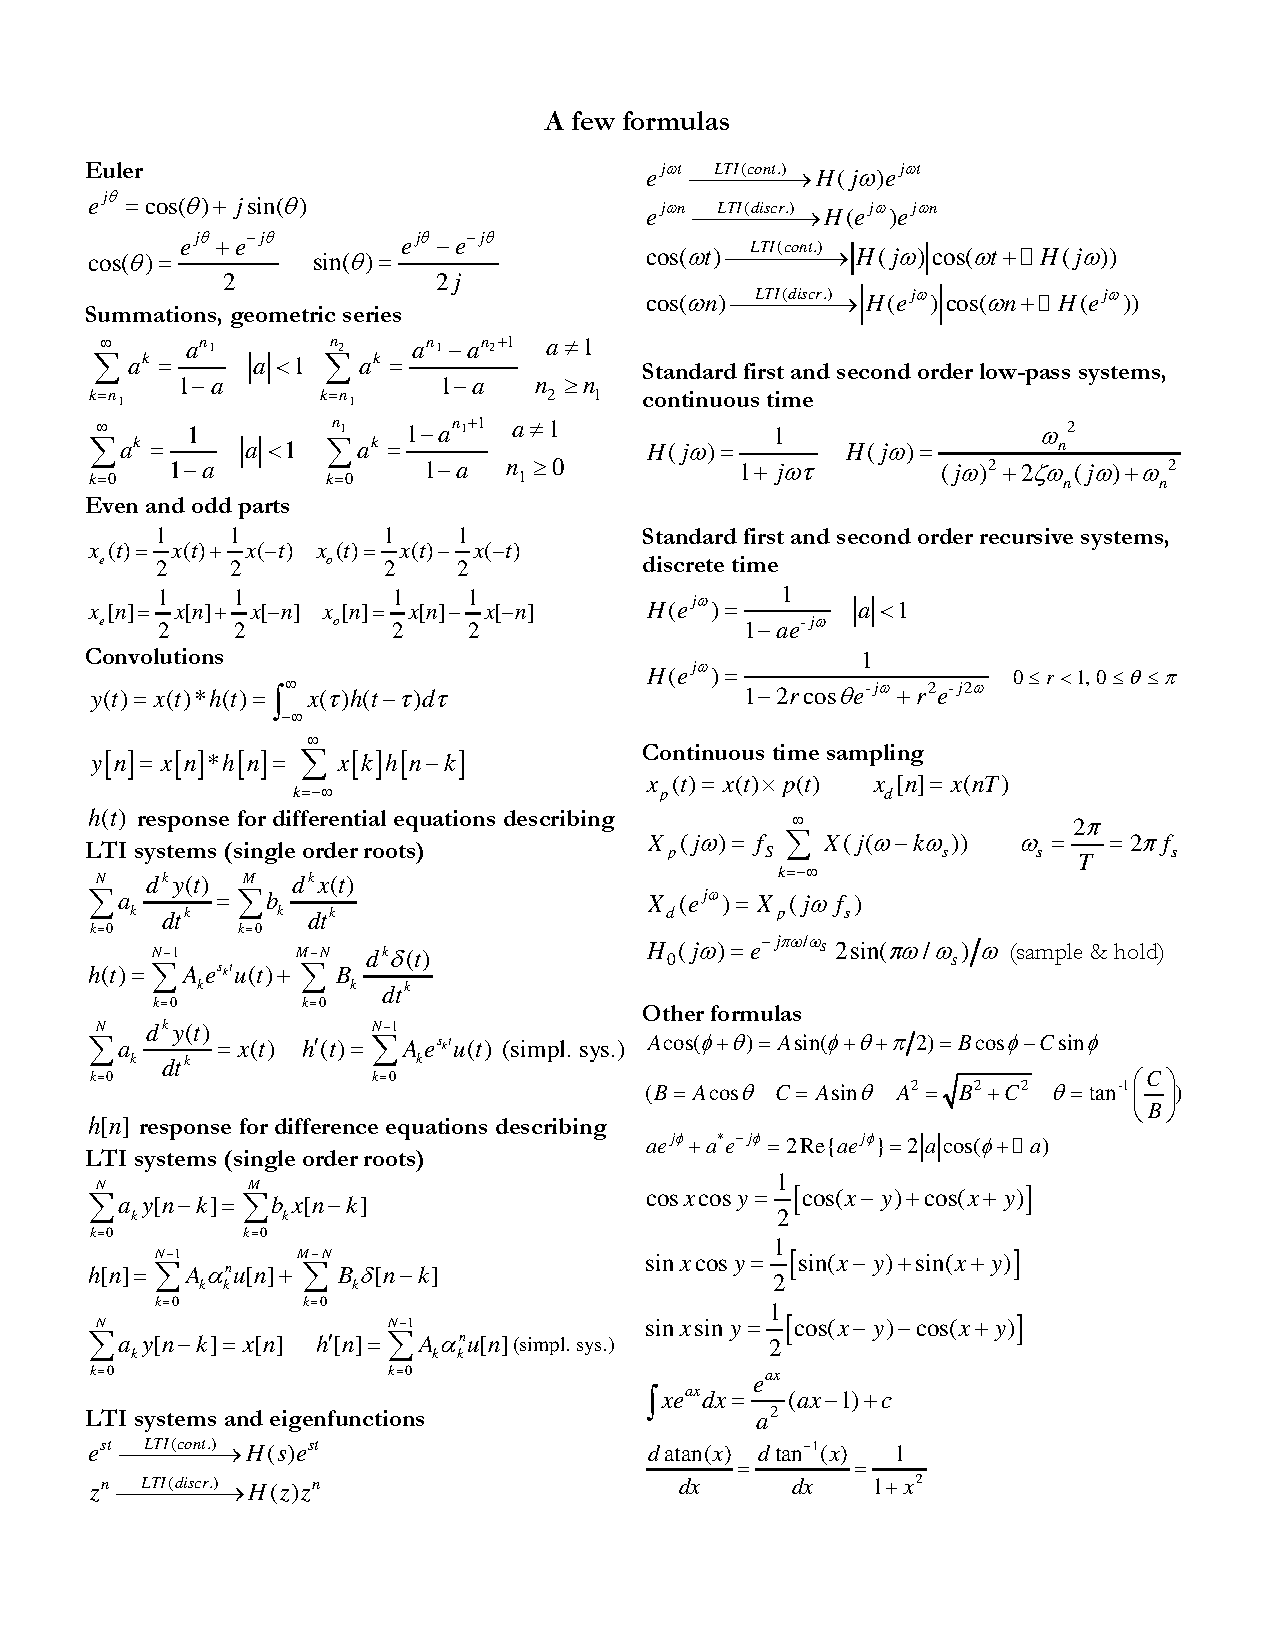
\includepdf[pages=-]{Formula-Sheets}
\end{document}